\documentclass[oneside,11pt]{book}


\textwidth=6.5in \textheight=9.0in \oddsidemargin=0in \evensidemargin=0in
\topmargin=-.5in \headheight=0.3in \headsep=0.2in \footskip=0.2in
%%\topmargin=0in \headheight=0.5in \headsep=0.2in \footskip=0.2in
\usepackage {amssymb}
\usepackage [fleqn]{amsmath}
\usepackage {graphicx}
\usepackage {verbatim}
\usepackage {longtable}
\usepackage {listings}
\usepackage{enumitem}

\usepackage[table,xcdraw]{xcolor}
% \usepackage[ruled,vlined]{algorithm2e}
\usepackage{ragged2e}
\usepackage{algorithm}
% \usepackage{algorithm2e}

\usepackage{algpseudocode}

\newcommand{\doctype}{Report}
\newcommand{\doctypeshort}{Report}
\newcommand{\kernelName}{Random Walk}
\newcommand{\doctitleshort}{\kernelName}
\newcommand{\doctitlelong}{Distributed Random Walks on Dynamically Weighted Graphs}
\newcommand{\chapterAuthor}{Trenton W. Ford}
\newcommand{\docnumber}{}
\newcommand{\docversion}{1.0}
\newcommand{\originaldate}{9-26-2018}
\newcommand{\modifieddate}{\today}
\newcommand{\myInitials}{TF}

\graphicspath{{figures-RW/}} %sets path to figures directory

\lstset{
    basicstyle=\small\ttfamily,
    %language=matlab,i
    frame=tb,
    tabsize=2, 
    showstringspaces=false, % don't mark spaces in strings
    numbers=left, % display line numbers on the left
    commentstyle=\color{green}, % comment color
    keywordstyle=\color{blue}, % keyword color
    stringstyle=\color{red} % string color
    %framexleftmargin=0.25in,
    xleftmargin=0.25in,
    columns=flexible}

\usepackage{color}
\usepackage{tikz}

% Tikz settings optimized for causal graphs.
% Just copy-paste this part
\usetikzlibrary{shapes,decorations,arrows,calc,arrows.meta,fit,positioning}
\tikzset{
    -Latex,auto,node distance =1 cm and 1 cm,semithick,
    state/.style ={ellipse, draw, minimum width = 0.7 cm},
    point/.style = {circle, draw, inner sep=0.04cm,fill,node contents={}},
    bidirected/.style={Latex-Latex,dashed},
    el/.style = {inner sep=2pt, align=left, sloped}
}

\usepackage{makeidx}
\makeindex

\usepackage{fancyhdr}
\pagestyle{fancy} \fancyhead{}

%\chead {\doctypeshort:\doctitleshort}
\chead {\doctitleshort}
%\rhead{Version \docversion}
\lfoot{Version \docversion}
\cfoot{}
\rfoot{\thepage}
\renewcommand{\headrulewidth}{0pt}

%added to increase depth of TOC
\setcounter{secnumdepth}{4}
\setcounter{tocdepth}{4}


\bibliographystyle{plain}

\begin{document}
\setcounter{page}{1}
\pagenumbering{roman}

\begin{comment}
% Following is commented out
\begin{titlepage}
\begin{center}
{ \LARGE \bf \noindent \doctype}

\par { \LARGE \bf \noindent \doctitlelong}
\vskip 0.5in
{\LARGE \bf \noindent \chapterAuthor}
\vskip 0.5in
{\large \bf \noindent Version \docversion}
\vskip 0.5in
{\large \bf \noindent \modifieddate}
\end{center}

\end{titlepage}

\end{comment}

%\tableofcontents

%\listoffigures

%\listoftables

\newpage
\setcounter{page}{1} \pagenumbering{arabic} \rfoot{Page \thepage}

\chapter{\doctitlelong}\label{sec:gl-kernels}
\begin{center}
    Contributed by \chapterAuthor
\end{center}

%\section{This is a Dummy Readme Section}\label{sec:sample-\myInitials}

Please read this section to understand what to do for your CSE 60742 graph kernel paper, how your ``standalone'' paper will be integrated into a class \textbf{Compendium of Graph Kernels} report that is part of an NSF project, and how at the end you are encouraged to use it as the starting point for an independent publication.

\subsection{Use as a Test File}
The first time a copy of this package is compiled, the following text should be converted correctly:

\begin{itemize}[noitemsep,nolistsep,leftmargin=*]

\item This section reference, Section \ref{sec:sample-\myInitials}, is a dummy section to allow you to verify you have imported the template correctly.

\item This section reference, Section \ref{sec:sequential-scaling-\myInitials}., should  properly refer to the Sequential Scaling section: 

\item Citation \cite{6567199} should be to a paper called ``Comparative performance analysis of a Big Data NORA problem on a variety of architectures'' and be listed in the bibliography.

\item There should be a table labelled Table \ref{tab:bluegene-\myInitials} that has characteristics of a Blue Gene computer.

\item Fig. \ref{fig:xyz-\myInitials} should properly refer to a figure called ``Characteristics of Blue Gene Computers'', created from a file``sga-benchmarks.pdf'' from directory ``figures-xxx''.

\item Algorithm \ref{alg:J2} should be some pseudo-code for an algorithm named ``Incremental Jaccard.'' (This pseudo-code uses the algorithm and algpseudocode packages.)
\end{itemize}


\begin{table}\begin{centering}
  \centering
  \begin{tabular}{|c|c|c|c|c|}
    \hline
Parameter&L&P&Q&Q/P\\
\hline\hline
Cores/node&2&4&16&4X\\ \hline
Core Clock (GHz)&0.7&0.85&1.6&1.9X\\ \hline
Max Node Memory (GB)&1&4&16&4X\\ \hline
Memory Ports per Node&1&2&2&same\\ \hline
Memory B/W per Port&5.6&6.8&21.35&3.1X\\ \hline
Total Memory B/W (GB/s)&5.6&13.6&42.7&3.1X\\ \hline
Inter-node Topology&3D&3D&5D&\\ \hline
Links per Node&12&12&22&4.7X\\ \hline
Bandwidth per Link (GB/s)&0.175&0.425&2&4.7X\\ \hline
Total Link B/W (GB/s)&2.1&5.1&44&8.6X\\ \hline
  \end{tabular}
  \caption{BlueGene Family Characteristics.}
  \label{tab:bluegene-\myInitials}
\end{centering}\end{table}

\begin{figure}\begin{centering}
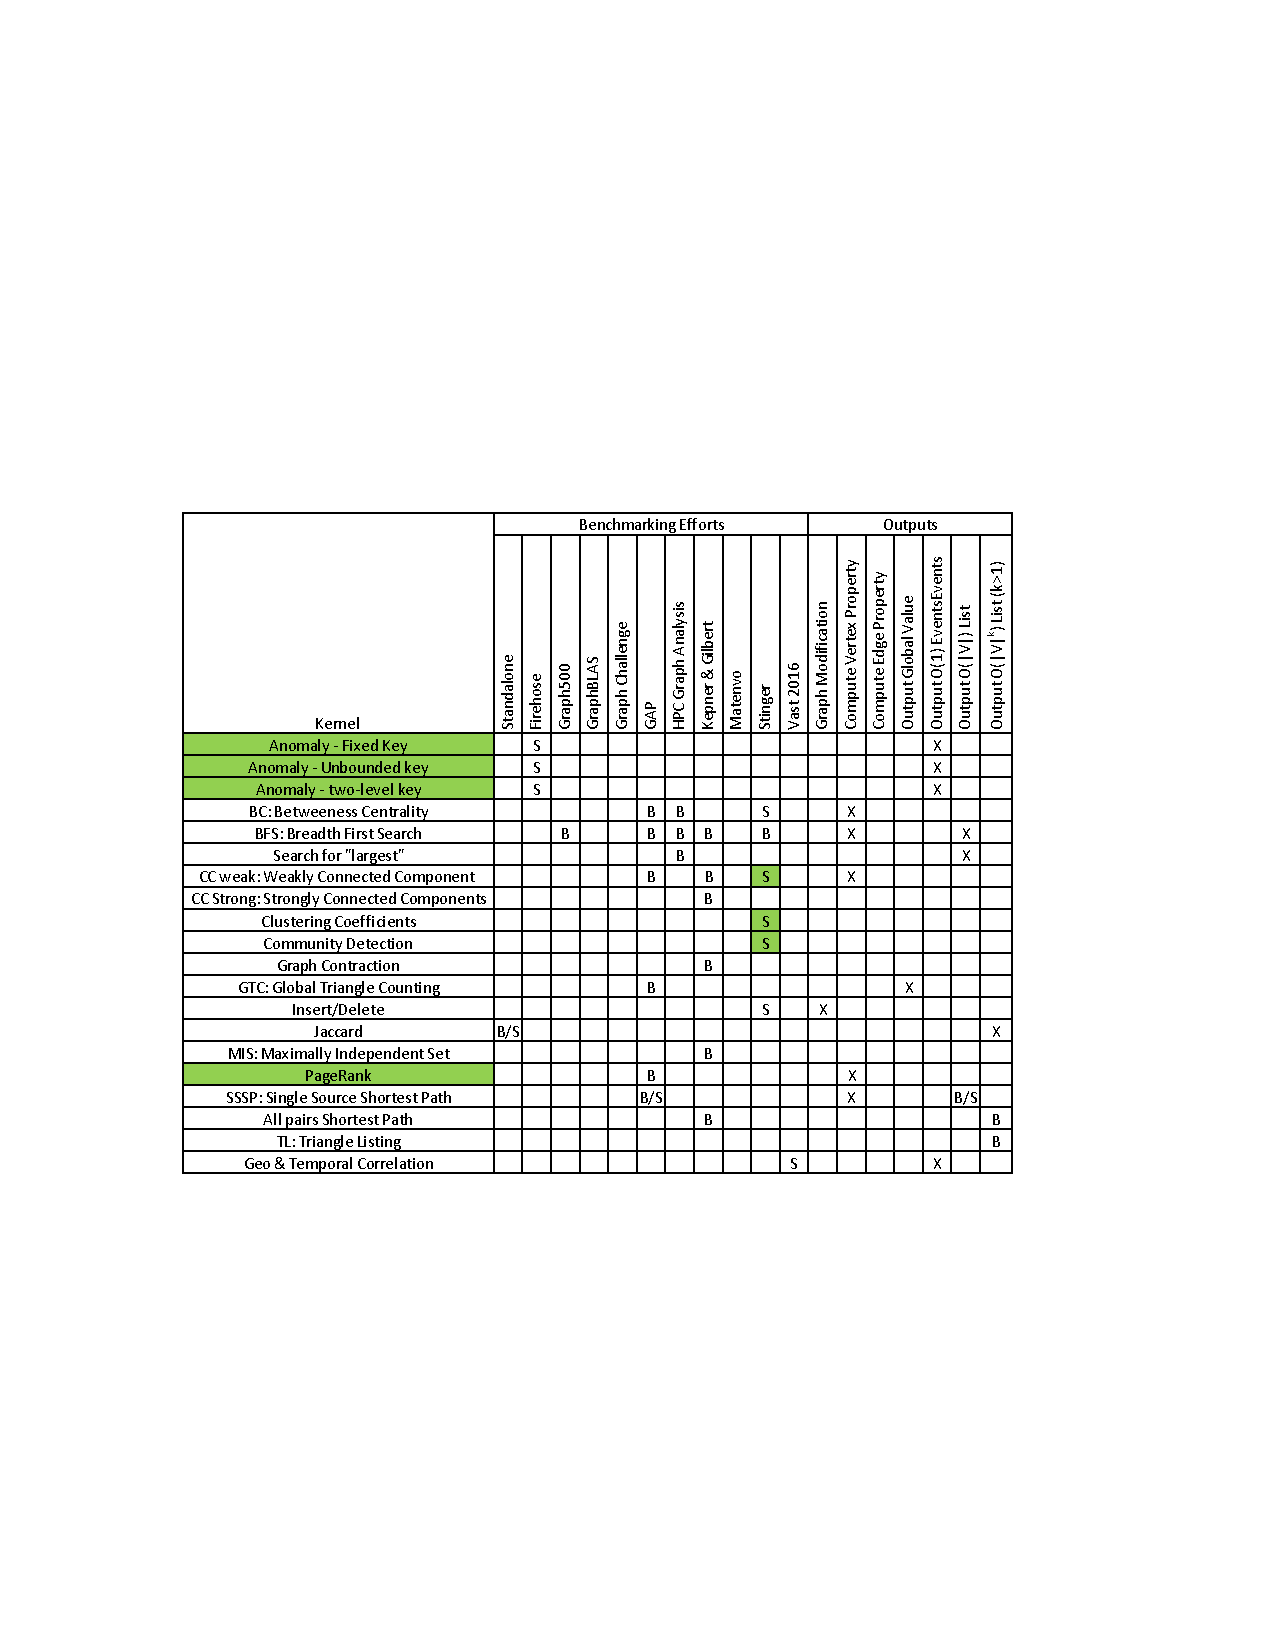
\includegraphics{sga-benchmarks.pdf}
\caption{Characteristics of Blue Gene Computers.}
\label{fig:xyz-\myInitials}
\end{centering}\end{figure}

\begin{algorithm}
\caption{Incremental Jaccard: 
\newline $L,~R,~E$ as above
\newline $N(u)~=~\{w|(G)$ in $E\}$}
\label{alg:J2}
\begin{algorithmic}[1]
	\Procedure{J2(u, v)}{}
    \For{$u$ in $L$}
    	\For{$v~>~u$ in $L$}
    	    \State $\gamma[u,v]~\gets~0$
    	    \For{$w$ in $N(u)$}
    	        \If{$w$ in $N(v)$}
    	            \State $\gamma[u,v]~+=~1$
    	        \EndIf
    	    \EndFor
    	    \State \textbf{end for}
		\EndFor
		\State \textbf{end for}
	\EndFor
	\State \textbf{end for}
	\EndProcedure
\end{algorithmic}
\end{algorithm}

\subsection{README}

This package, when personalized by a student in CSE 60742, will generate a pdf formatted as a ``Chapter.'' In general, files in the ``figures-xxx'' directory are the figures for this paper. Files in the  ``text-xxx'' directory are the .tex source latex files for the paper, with each file representing a separate section. Each current file starts with a $\backslash$section and the name of the section. A label is given for that section in a standard format of ``sec:\textit{filename}-xxx''. The ``refs-xxx.bib'' is a .bib (bibtex) file holding all references.

The latex organization of this package will allow the instructor to ``easily'' compile multiple such student papers into a single "Compendium of Graph Kernels" report, with each student paper a separate chapter, and each having a similar look and feel. However, it is certainly my goal to encourage students to take their individual ``chapters'' and adapt them to conference or journal submissions with minimal effort. So please follow the directions below.

\subsection{Initial Setup Instructions}

After down-loading a copy of this package, each student should do the following:

\begin{enumerate}[noitemsep,nolistsep,leftmargin=*]

\item Upload the package to a new project in ShareLatex with the  name ``\textit{xxx-ijk}''where ``\textit{xxx}'' is a mnemonic or abbreviation for the graph kernel you studied and ``\textit{ijk}'' is a 3-letter initials of your name. If you are creating multiple chapters, add a number or something to the initials to distinguish between the papers. The goal is to end up with a unique latex project name. An example might be ``BFS-PMK''.

\item Change the ``xxx'' in the names for directories "figures-xxx" and "text-xxx", and the file ``refs-xxx.bib'' to the same kernel abbreviation.

\item In the ``text-xxx$\backslash$body.tex'' file, change all ``xxx'' to the kernel abbreviation.

\item In the ``ChapterHeader.tex'' file, change the ``xxx`` in the last line to the kernel abbreviation.

\item In the ``text-xxx$\backslash$redirects.tex`` do the following first:
    \begin{itemize}[noitemsep,nolistsep,leftmargin=*]
    \item Change ``My Name'' to your name as yo want listed as author.
    \item Insert a short 1-word name in the newcommand for kernelName to reflect what kernel you discuss in the paper. It can be the same as your abbreviation.
    \item Change the ``xxx`` in the ``$\backslash graphicspath$'' line to the kernel abbreviation.
    \item Insert a longer title as desired in the newcommand for doctitlelong to reflect what this chapter should be called (reflect a key application that would use your kernel and an expanded name for the kernel, such as ``Graph Exploration - Breadth First Search'').
    \item Insert the date of your first version of the paper in the newcommand for originaldate.
    \end{itemize}

\item In line 84 of main, change ``xxx'' as above.

\item Check if the whole package still compiles, and look thru the ``This is a Sample Section'' to see if all references still worked properly.

\item In the "text-xxx$\backslash$body.tex" file, comment out the "Sample" section with a leading \%. (Leaving it in the directory may given you some sample latex formats to copy and paste).

\item Recompile to ensure it still all works. The first section should now be ``Introduction''.

\item You are free to delete the entries in the .bib file.

\item Please ``share'' your project with kogge@nd.edu

\item You are now free to add text.
\end{enumerate}

\subsection{When Filling in Your Own Text}

\begin{enumerate}[noitemsep,nolistsep,leftmargin=*]
    \item PRETEND VERY HARD that what you write will turn eventually into a submission for a conference or journal like KDD. As such, feel free to discuss with your advisor, move sections around, add additional sections as needed, etc. The structure of this latex is to allow you to take the files in the ``text-xxx'', ``figures-xxx'', and ``refs-xxx.bib'' and with little work, plug it into whatever is the main latex template specified for your conference. In particular you should be able to simply insert a reference to the body.tex file into the conference template and have everything port.
    
    \item Also for the class compendium report feel free to add appendices that give more detail.
    
    \item When starting to add text to a section, delete or comment out the paragraph of text I included.
    
    \item Given I expect this paper to evolve over the semester, feel free to comment out from the body file any $\backslash$input line for a section you are not modifying right now. You can uncomment it when you go back to add text.
    
    \item Place any new text files you generate in the ``text-xxx'' directory.
    
    \item Feel free to use the Figure and Table sample above as cut and paste as needed.
    
    \item End each label with ``-xxx'' where ``xxx'' is your initials. You could also use the ``-\myInitials'' for this so you don't have to remember your initials. This helps avoid accidentally duplicate labels when multiple chapters are combined.
    
    \item It is not required, but when labelling something, I use a prefix of ``sec:'' for sections, ``fig:'' for figures, ``tab:'' for tables, etc.
    
    \item If you would like to see a table of contents, figures, or tables, uncomment the lines in ``main.tex'' (remove the ``\%'').
    
    \item Note that I used ``[noitemsep,nolistsep,leftmargin=*]'' when starting a list to remove both the initial indent and remove extra lins around each item. This is to compact the text as one might do for a page-limited conference paper.
    
    \item The latex packages \textit{algorithm} and \textit{algpseudocode} are great for writing pseudocode.
    
    \item In terms of writing, my graduate advisor insisted on ``present tense and active voice'' - it results in shorter, clearer, and more readable text. A reference that all of you should have at your elbow is \cite{strunk1999elements}. You can get this from Amazon for under \$2,

\end{enumerate}

\subsection{Paper Development Schedule}

You will develop your paper in three phases over the semester.
\begin{enumerate}
    \item A starting point consisting of a first cut of the Introduction through the Key Graph Kernel, but not including any implementation.
    \item An extension covering a reference sequential implementation. This version may be in something as simple as Python.
    \item A final extension covering either some sort of an initial parallel implementation or a major revision of the sequential implementation.
\end{enumerate}

At any point, with permission of instructor, if you hit a wall, and want to switch to a different kernel, that can be worked out.

Twice during the semester (after each of the first two passes), each student will both perform  two reviews of other papers, and receive three reviews back (two other students and the instructor). This will ensure you learn in detail a bit more about at least four other graph applications and kernels, and get feedback on your own paper that you can use to improve it. Such give and take will be invaluable as you continue in your graduate research. On each review cycle you will receive a ``randomly selected'' paper to review, and can choose the other one to review (no repeats and first come first choose when choosing). You will be expected to at least consider each set of reviews in your next revision.

Although actual projects and papers are to be done individually, please feel free to collaborate on graph generators and locating and downloading data sets. If at all possible a common data format such as ``'csv'' make for an easily interchangeable and processable format.

When you port this to a conference template, delete the file ``ChapterHeader.tex, main.tex, and redirects.tex.'' You can also if you want delete the ``sample.tex'' file from the ``body'' directory. You now need only insert a ``$\backslash$input$\{text-xxx \backslash body\}$ into your new template where the body text should go.

    

\section{Introduction}\label{sec:introduction-\myInitials}

% Provide an introduction to the problem area(s) for which the kernel you want to study is relevant. For this chapter, you DO NOT need to discuss why graphs are important in general, what graphs are, or other ``common'' things like how to represent graphs. Such things will be addressed in a common part of the Compendium report. Clearly, though, when you convert your chapter into a paper you will have to add a bit of such stuff back into the intro, and perhaps elsewhere.

In 2014 the world saw the most massive resurgence of the Ebola virus in history. The epidemic was mainly localized to West Africa but spread to other parts of Africa, and even other countries through a myriad of transportation methods. All told, nearly 30,000 people were infected worldwide, of which 11,300 died. These numbers are terrible, but they could have easily been worse. A large part of planning against the transmission of epidemics is in modeling the dispersal of infection through physical travel networks. In 2014 this modeling helped the Centers for Disease Control (CDC) increase monitoring on select ports to slow or prohibit the possibility of widespread transmission. The goal of this paper is to investigate models of disease transmission that utilize Random Walks as their underlying kernel. 

\section{The Problem as a Graph}\label{sec:asgraph-\myInitials}

% Discuss here how instances of that problem can be expressed as a graph.

We can formalize the above problem as a complex, heterogeneous network. With the following structure:

\begin{center}
    \parbox[t]{2.4in}{
        \raggedright%
        \textbf{\textit{Node Types :}}
        \begin{enumerate}[topsep=0pt,itemsep=-2pt,leftmargin=13pt]
            \item Airport
            \item Seaport
            \item Rail Station
        \end{enumerate}
    }%
    \parbox[t]{2.4in}{
        \raggedright%
        \textbf{\textit{Edge Properties :}}
        \begin{enumerate}[topsep=0pt,itemsep=-2pt,leftmargin=13pt]
            \item Direction
            \item Transition Probability ($p_1...p_k$)
            \item Distance
            \item Travel Time
        \end{enumerate}
    }
\end{center}

\begin{figure}
    \centering
    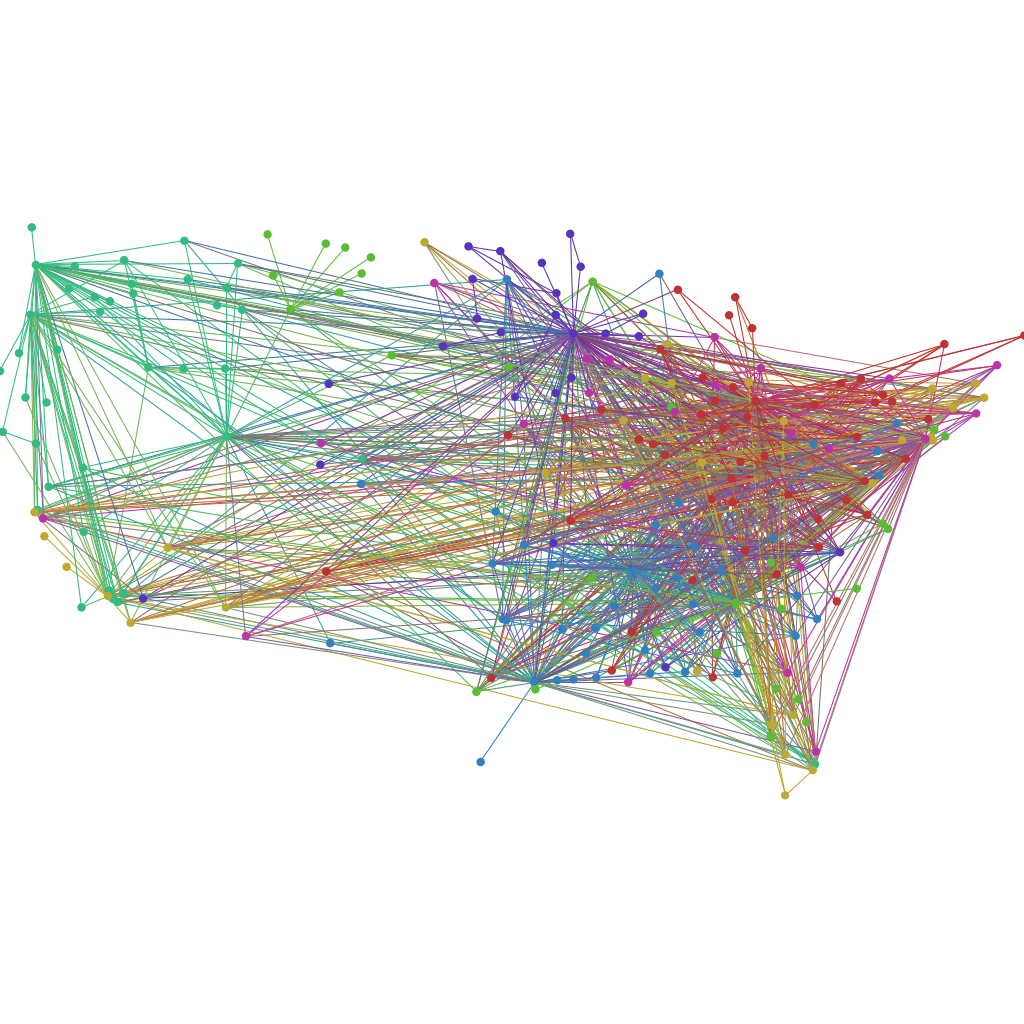
\includegraphics[width=1.0\textwidth]{figures-RW/usairport_base.png}
    \caption{US Domestic Airport Network\cite{stanford_dhs}}
    \label{fig:us_domestic}
\end{figure}

\newpage
Figure \ref{fig:us_domestic} shows a network containing only nodes of type \textit{airport}, with edges weighted and colored by the frequency of travel between two airports.



\section{Some Realistic Data Sets}\label{sec:basic-datasets-\myInitials}

\subsection{Example Data Sets}

\begin{table}[h]
    \centering
    \caption{Real-world datasets and their sizes.}
    \\
    \begin{tabular}{lll}
        % \multicolumn{3}{c}{{\color[HTML]{343434} \textbf{Potential Datasets}}}\\
        \hline
        \multicolumn{1}{|l|}{\textbf{Dataset}}  & \multicolumn{1}{l|}{\textbf{Approx Vertices}} & \multicolumn{1}{l|}{\textbf{Approx Edges}}   \\ \hline
        \multicolumn{1}{|l|}{DOT Railway Data}  & \multicolumn{1}{r|}{196K}           & \multicolumn{1}{r|}{250K} \\ \hline
        \multicolumn{1}{|l|}{SNAP Airport Data} & \multicolumn{1}{r|}{456}            & \multicolumn{1}{r|}{71K}       \\ \hline
        \multicolumn{1}{|l|}{KNB Shipping Data} & \multicolumn{1}{r|}{3700}     & \multicolumn{1}{r|}{15K}       \\ \hline
    \end{tabular}
    \label{table:potential_datasets}
\end{table}

Transportation networks, in general, are pretty ubiquitous. The SNAP Labs\footnote{\cite{snapnets}https://snap.stanford.edu/data/reachability.html} usually maintain stable data repositories for network data, and here is no exception. The \textbf{Airline Travel Reachability Network} contains both US and Canadian airport travel nodes and edges, including plenty of metadata such as travel time, geodata, and other potentially useful things. 

Maritime data is more difficult to find, but there are multiple years worth of shipping data maintained by The Knowledge Network for Biocomplexity (KNB)\cite{knb_data}, and increasing amounts of data in this space is becoming open access. Railway datasets are less convenient as the datasets are generally maintained by the respective governments for which the railway belongs. For instance, US railway data can be found at either Data.gov, or the Department Of Transportation data page\footnote{osav-usdot.opendata.arcgis.com/}.The size and order of these datasets can be found in table \ref{table:potential_datasets}.

\subsection{Constructing A Complex Network}

If we were to construct a complex network from the above transportation network datasets, we would find that the size and order of the network would increase greatly. For instance, if an airport terminal also contains a train terminal (not irregular) then the airport and train station nodes must either merge, or copy the inbound and outbound edges of their counterpart. This sort of node merging or edge duplication activity results in quite irregular networks. This irregularity, coupled with the network's heterogeneity, makes it difficult to build network generators that sufficiently capture the depth of interactions and metadata represented in real-world data.

Moreover, as stated above, many of the datasets are maintained by separate entities and represent transportation networks that serve different goals. For instance, the difference between passenger trains and freight trains means a great deal when attempting to capture human vectored disease transmission. For these reasons, interested parties such as the World Health Organization (WHO) and the CDC are working with countries all over the world to increase the accuracy of and access to this data.

\subsection{Generating Representative Datasets}
Given the difficulties discussed above related to wrangling the real-world datasets, we chose to use synthetically generated datasets of several types. We used several sizes of grid networks where vertices were given random initial populations, the edges outgoing from a vertex is set as a proportion of the vertex population and out degree. A vertex is then selected at random and some small portion of their population is infected initially.

When using graphs that are not grid structured, Erdős–Rényi for example, because the vertex degrees is irregular we use them to inform the vertex population size. Greater degree vertices have greater population sizes. A vertex is still selected to have an initial infected population, but instead of random uniform sampling, the sampling is weighted by vertex population. Higher population vertices are more biased towards having the initial observed infective population. 

We plan to investigate other real-word adjacent graph generation techniques in further work.

\section{\kernelName -A Key Graph Kernel}\label{sec:problem-\myInitials}

% Discuss here what a graph kernel that can help solve such problems might be. Pseudo code is fine, but in enough detail that you can project time and space complexity. Discuss also what sort of performance metric makes sense.

When a problem can be represented as a graph, a simple random walk on that graph represents unbiased movement through the graph where only structure is considered. For this reason, random walks are often used to determine if real observed traversal through a network is being influenced by non-structural factors. In this way, random walks serve as a traversal baseline given no prior knowledge of the graph. 

Given a graph $G(V,E)$ where $V$ is a set of vertices and $E$ is a set of edges for which an edge $(u,v) \in E \iff u, v \in V$ if edge $(u,v)\inE$ then vertices $u$ and $v$ are said to be adjacent. A random walk on a graph $G$ is a sequence $S$ of adjacent vertices, where for any vertex in the sequence $s_i$, vertex $s_{i+1}$ is chosen at by some heuristic, normally uniform random selection, from vertices adjacent to $s_i$. 

Using the above described random walk as a baseline, we can tailor a random walk to model our problem by specifying the heuristics our walk will use to select an adjacent vertex to traverse. To test whether our heuristic appropriately models our specific application, we can attempt to replicate a previously observed real-world occurrence of our application. The closer we are able to get the model to approximate real-world observations the better. We can iteratively modify the model heuristics to better fit observations using several methods (gradient descent, grid search, etc.). Using this simple process a random walk model can be built to fit our application. Once a good model is trained the goal would be to use the model to make predictions about unobserved occurrences. In our specific application we would want to use the model to make predictions about epidemic transmission for future disease outbreaks. In the disease transmission scenario described above, probabilistic random walks are used to represent individuals (infective or susceptible) moving through travel networks.

Unfortunately, in the real world infective individuals don't just traverse through a network. As infective individuals move through a network there are contagion characteristics to consider. Disease specific factors that a high-fidelity model would need to consider are:
\begin{center}
    \title{Disease specific model factors}
    \parbox[t]{2.4in}{
        \raggedright%
        \begin{itemize}[topsep=0pt,itemsep=-2pt,leftmargin=13pt]
            \item Carrier Proportion
            \item Incubation time
            \item Infective Duration
        \end{itemize}
    }%
    \parbox[t]{2.4in}{
        \raggedright%
        \begin{itemize}[topsep=0pt,itemsep=-2pt,leftmargin=13pt]
            \item Infectivity
            \item Transmissibility 
            \item Mobility Index
        \end{itemize}
    }
\end{center}

% \begin{itemize}
%     \title{Disease specific model factors}
%     \item Carrier Proportion
%     \item Incubation time
%     \item Infective Duration
%     \item Infectivity
%     \item Transmissibility 
%     \item Mobility Index
% \end{itemize}

Many of these factors require their own statistical models for best approximations. For our sequential and enhanced implementation we will keep our model model as simple as reasonable to test benchmark our solutions as comparably as possible. More clearly stated, the statistical support that would enable consideration of these disease specific factors are computationally expensive and rely heavily on pseudo-random sampling. Not only would this type of sampling increase the computation time of our implementations, but it would introduce a great deal of uncertainty into our results. The factors this implementation will consider are discussed in Section \ref{sec:sequential-algorithm-\myInitials}.

\subsection{Computational Bottleneck}

Consider the given application. If one wanted use a random walk based algorithm to model epidemic transmission within a real-world travel network then none of the individual data sets referenced above would be sufficient. People use many modes of transportation, and often mix modes during travel. Merge any two travel networks together and it quickly becomes apparent that the number of vertices may be linear, but the number of edges and the overall complexity of the resulting network increases exponentially.
One of the most powerful motivations for using random walk based algorithms is their speed, but the network sizes and complexity means that a random walk sequence may need tens of billions of steps model a scenario, and that process is repeated until goodness of fit is reached. Refining a model on a network of this scale is time prohibitive.

In the general case of random walks the computation time can be reduced using an ``embarrassingly parallel" variant of the algorithm that runs separate walks on different copies of the same graph using many different compute nodes simultaneously. When the individual compute nodes reach a stopping point their results are gathered and merged into a final product. Unfortunately in the epidemic transmission specific random walk an embarrassingly parallel implementation does not exist. Because our random walker carriers information that could change the underlying network, means that the graph is not guaranteed to be consistent across the individual compute nodes.

Considering these facts the obvious option is to do away with different compute nodes operating on copies of the graph, and have them work on the same copy simultaneously. This method introduces the problems of compute node memory consistency and coherence. Fortunately, there is another strategy. 

\subsection{Proposed Solution}

This research proposes to parallelize a random walk based epidemic transmission model across many compute nodes by partitioning the original network and distributing said partitions to the memory associated with individual compute nodes. Each compute node will be responsible for operations relating to the vertices within the partition of the graph allocated to it, and the outgoing edges associated with those vertices. This method still introduces the need for compute nodes to communicate when . Parallel Boost Graph Library extend the random walk kernel using a network specific distribution scheme that considers the interconnectedness of the network to determine how to distribute the network to compute nodes maintaining their own random walkers, and suggests an optimizing function to shift or duplicate nodes based on the minimization of communication.

\subsubsection{Network Partitioning}

Unlike the standard parallel random walk algorithm, we cannot arbitrarily partition our graph and distribute the partitions to distinct compute nodes and merge their individual results. The dynamism of the disease transmission random walk algorithm requires that changes to the underlying network such as edge and vertex properties are expected. Moreover, the compute nodes themselves can change the underlying graph attributes. Optimally done, this partitioning would minimize the number of messages passed between distributed random walkers. To approximate this optimal partition, metrics such as min-cut and spectral clustering will be tested in small networks against a baseline of randomly distributed nodes.

\subsubsection{Communication}

Communication will be handled by the Parallel Boost Graph Library's process group. I'll expand upon this in the next revision. 



\section{Prior and Related Work}\label{sec:related-\myInitials}

% This is space to add in discussion of \textbf{prior work} - word on the same problem or kernel that your paper assumes, and \textbf{related work} - work on the same application but using different approach or kernel, or a different but similar application..

Forthcoming.

\section{A Sequential Algorithm}\label{sec:sequential-algorithm-\myInitials}

\justifying{

One of the major advantages of the random walk process is that it is easy to understand in the uniformly weighted, non dynamic case. The algorithm is relatively simple. The input is a graph $G(V,E)$ where the edges $e \in E$ have associated weights, or transition probabilities $w_i$. If we consider a simple case where we select one starting vertex say $u$, and wish to perform a random step we would consider all adjacent vertices, say $x_1 \ldots x_k$, connected to $u$ over edges $e_1 \ldots e_k$, with associated weights $w_1 \ldots x_k$. Before taking a step, the weights of the adjacent vertices must be normalized as follows: 

\begin{center}
    $$p_i = \frac{w_i}{\sum_1^k{w_i}}$$
\end{center}


Where each of the $p_i$ will represent the probability of traversing across a given edge $e_i$. Given the normalization process, we are guaranteed that the probability of all adjacent edges will sum to 1, so we can use a standard uniform random number generator to sample from the edges. At that point we may successfully take a step. We can take as many of these steps as are available, and upon completion we are returned a vector containing the path of the random walk, starting with vertex $u$.
\par
\begin{algorithm}[H]
\SetAlgoLined
\KwData{Graph $G(V,E)$}
\KwResult{Path Of Random Walk}
 Select A Start Node $u$ Randomly\;
 Initialize path vector P.append($u$)\;
 \While{True}{
    edges=$u$.adjacent\;
  \eIf{edges.length $>$ 0}{
   edges.prob = normalize(edges.weights)\;
   $u$ = uniformSelect(edges.prob)\;
   P.append($u$)\;
   }{
   \textbf{return} P\;
  }
 }
 \caption{Simple Random Walk}
 \label{alg:simple_rw}
\end{algorithm}
}

\section{A Reference Sequential Implementation}\label{sec:sequential-implementation-\myInitials}

The current sequential implementation generates grid networks due to their regular network structures as the order of the network increases. The aim of this grid based implementation is to regularize the scaling results and make easier the comparison between the sequential and the parallel implementations of the disease transmission model.

% Get the correct citation for the paper
For the sequential representation, our implementation will roughly copy that put forth by Kelker in 1973\cite{Kelker1973}. Modifications were to increase the accuracy of the model by allowing the three variables ($\lambda$, $\mu$, and $p$) to be samples from non-uniform distributions. We also allow graphs that are not grids. Kelker's simulation model was the groundwork for more recent epidemic transmission simulations, but the complexity that they add to the random walk process makes it difficult to do meaningful complexity analysis of the algorithms. 

We also adopt Kelker's stopping criteria, in that we run the model until all of the individuals reach a homogeneous state. That is to say that either all people are infective, or all people are susceptible. Reasonable thresholds can be used instead of absolute convergence, but for the parameters that we set, absolute convergence should always be possible. 


\section{Sequential Scaling Results}\label{sec:sequential-scaling-\myInitials}

% Discuss here results from your sequential implementation. Include software and hardware configuration, where the input graph data sets came from, and how input data set characteristics were varied. Did the performance as a function of size vary as you predicted?

For readability, these results have been broken into sections based on a given stopping criteria.

\subsection{Stopping Criteria: BFS}
\subsection{Stopping Criteria: DFS}
\subsection{Stopping Criteria: Vertex Cover}
\subsection{Stopping Criteria: Mixture}

When discussing the scaling results of the sequential random walk implementation, what must first be imposed is a \textit{stopping criteria}. Without a stopping criteria a random walk has no definite end state. For the purposes of the results here, the algorithm will stop once all nodes have been visited at least once, also known as the \textit{node cover} stopping criteria. Even with this imposition, it has been shown that the speed of random walks changes with the structure of the network being traversed\cite{Virág99onthe}. This limits the inferences that can be gleamed from the results from different graphs in relation to each other, but during the parallel implementation results analysis we can compare the two algorithms directly over each of the networks.

Results from the sequential implementation are forthcoming, dealing with some slippery errors during optimization.

\section{An Enhanced Algorithm}\label{sec:enhanced-algorithm-\myInitials}

% Discuss here the outlines of an enhanced algorithm. This could be a parallel code, a code with some significant heuristics, or a code written in a non-traditional programming paradigm. Pseudocode is fine. Discuss what you think is the computational complexity.

Forthcoming.

\section{A Reference Enhanced Implementation}\label{sec:enhanced-implementation-\myInitials}

% Discuss here an implementation of the enhanced algorithm. Include what language/paradigm you used for the code.

Forthcoming.

\section{Enhanced Scaling Results}\label{sec:enhanced-scaling-\myInitials}

% Discuss here results from the enhanced algorithm. Include software and hardware configuration, where the input graph data sets came from, and how input data set characteristics were varied. Ideally plots of performance vs BOTH problem size changes AND hardware resources are desired. Did the performance as a function of size vary as you predicted?

Forthcoming.

\section{Conclusion}\label{sec:conclusion-\myInitials}

% Summarize your paper. Discuss possible future work and/or other options that may make sense.

Forthcoming.

\section{Response to Reviews}

% This will be included only in the second and third iterations, and will be a summary of what you learned from the reviews you received from the prior pass, and how you modified the paper accordingly.



\bibliography{refs-RW}

\printindex

\end{document}
